%%
% The BIThesis Template for Bachelor Graduation Thesis
%
% 北京理工大学毕业设计(论文)第一章节 —— 使用 XeLaTeX 编译
%
% Copyright 2020-2023 BITNP
%
% This work may be distributed and/or modified under the
% conditions of the LaTeX Project Public License, either version 1.3
% of this license or (at your option) any later version.
% The latest version of this license is in
%   http://www.latex-project.org/lppl.txt
% and version 1.3 or later is part of all distributions of LaTeX
% version 2005/12/01 or later.
%
% This work has the LPPL maintenance status `maintained'.
%
% The Current Maintainer of this work is Feng Kaiyu.
%
% 第一章节

\chapter{绪论}

\section{研究背景}

区块链是一种分布式的共享账本,允许数个参与方一同共享数据。区块链技术所拥有的去中心化、透明性和安全性等优势,令这一新兴的概念迅速为各行各业接受:中国人民银行数字货币研究所正在积极探索区块链技术在低并发、低敏感的资产确权、交易转让、账本核对等场景下的应用\cite{shuYanSuo};区块链透明化的特点和极高的安全性也引起了地产行业的注意\cite{usageOfBC}。可以预见,区块链技术在未来将吸引更多行业加入,以其去中心化、不可篡改等特性造福人类社会。

树状区块链,是实验室正在开发并已趋于完善的改良型区块链。其基本思想大致为:将区块分为创世块、分支区块和叶子区块三种;结合GeoHash编码技术,不再采用传统区块链的单链结构,形成类似于字典树的树状结构;同时,为了满足快速查询的需要,在区块中增添了一些辅助数据结构。经过以上改良,树状区块链可以在对地理位置敏感、且网络结构变化较频繁的应用场景中,发挥相较传统区块链更好的理论性能。

车联网技术(Internet of Vehicle)属于物联网技术的范畴,其思想乃是在车辆上搭载接入网络的设备,旨在实现不同车辆之间的相互通信;不仅如此,车联网技术也容许车辆与行人、路边基站等交通参与方和交通基础设施通信,实现实时的车况检测、路况查询与收集等功能,对于提升车主用车体验、乘客出行体验有强大的潜力。2022年12月8日,公安部发布的数据显示全国机动车保有量到达4.15亿辆,机动车驾驶员人数超过5亿位!随着如何安全有效地管理如此庞大的保有量带来的海量数据这一巨大挑战变得日益严峻,人们纷纷将目光转移到了区块链上\cite{bcInIoV}。然而,传统区块链在处理车联网场景下的具体事务时,往往存在诸如此类的一些弊端:

\begin{itemize}
  \item 车辆作为区块链网络的参与者(节点)时,其地理位置可能发生很大变化,致使网络结构需要频繁更新;
  \item 传统区块链采用单链结构,在区块链上执行的查询时间复杂度较高;
  \item 在车联网系统中,车辆应该关心的信息大部分来自于其所在位置的临近街区,而传统区块链并不以地理位置索引区块及其交易,故一次查询可能会获得较多无用信息等。
\end{itemize}

由于树状结构相比单链结构的深度更小,且采用了与地理位置相关的GeoHash进行分支构造,故有效降低了查询开销,令基于位置的信息查询能够更加“有的放矢”,有望为运用区块链技术处理车联网问题提供合理可行的解决方案。

目前,实验室已有的树状区块链采用以太坊(Ethereum)实现。以太坊是一个开源的区块链计算平台,允许开发者进行去中心化应用程序(DApp)的开发和部署。其支持以Solidity编程语言编写运行在在以太坊虚拟机上的脚本程序(智能合约Smart Contract),极大拓宽了区块链的功能适用性。

Substrate是一组开源、模块化的区块链开发框架,允许开发者自由地使用官方预定义的各种组件构建个性化的区块链,并于其上使用基于Rust的ink!编程语言进行智能合约开发。与以太坊比较,Substrate具有包括而不仅限于如下优势:

\begin{itemize}
  \item 支持模块化设计,程序员可以轻松增删模块,构建更加贴近实际需求的区块链
  \item 采用Rust编程语言作为其底层实现,速度更快,效率更高
  \item 支持编译为大多数现代浏览器支持的WebAssembly二进制,提供了更好的跨平台兼容性
\end{itemize}

本文将在车联网的应用场景下,以实验室已有工作——出租车调度系统为例,探究树状区块链在不同工况下的性能表现,验证其拥有相较传统单链区块链更好的性能表现。本文还将积极尝试为将树状区块链从以太坊平台转向更优秀的Substrate平台。鉴于时间和笔者能力之限,本文仅讨论区域索引区块链的部分特性的迁移工作,此举旨在验证两平台在功能上的相似性,进而确保未来树状区块链的底层功能迁移工作的可行性。

\section{相关技术调研}

\subsection{区块链技术概述}

2008年,一位自称为中本聪的人发布了名为《Bitcoin: A Peer-to-Peer Electronic Cash System》的论文,宣告了区块链技术的诞生。区块链,乃是一个分布式的账本;区块链网络不存在所谓的“中心服务器”,每台参与构成区块链网络的计算机(又被称为“节点”)均持有一份该账本的副本。每一笔交易,都将记录在名为“区块”的数据结构中;随着区块的不断产生,它们将形成一条单向链状结构,且区块上存储的数据将不可再被修改。通过称为共识算法的机制,各节点能够就区块链的当前状态达成一致,并在链上数据发生变化时及时追踪并更新到自身存储的账本中。不仅如此,若某个节点尝试擅自修改自身所持有的账本,其行为会被共识算法拒绝,从而规避了恶意篡改链上数据的风险。上述区块链的优势,令区块链这一新兴的概念迅速吸引了各行各业的眼球。可以预见,区块链技术在未来将吸引更多行业加入,以其去中心化、不可篡改等特性造福人类社会。

\subsection{智能合约概述}

智能合约(Smart Contract)这一概念由Nick Szabo于1994年提出。在比特币的支付模型中,仅存在一个简单的堆栈计算机。由于其可用的操作方法并非图灵完备,只能执行比较简单的操作,从而限制了区块链的应用场景。智能合约的出现打破了这一局面。在Szabo于1996年撰写的《Smart Contracts: Building Blocks for Digital Markets》一文\cite{nickSzabo}中,Nick设想智能合约就是运行在区块链上的一段程序,当满足某种条件时,相应代码将自动被执行,而该过程人类无需也无法介入。智能合约一定程度上避免了交易双方抵赖的问题,并且其图灵完备的特性也令区块链技术在不同应用场景下的适应性大大增加了。

\subsection{区域索引区块链和树状区块链概述}

周畅设计的区域索引区块链,实现了区块链地理信息索引方法,能够依据地理位置信息快速查询特定位置的交易\cite{sensors}。如图1-1所示,相较以太坊官方实现的传统区块链而言,区域索引区块链在区块头中加入了区域状态树的树根哈希,以支持基于位置的快速信息查询;同时,为追踪每个账户的包括位置信息的完整状态,在账户状态数据结构中还加入了当前的地理位置字段、和账户位置树这一数据结构。不仅如此,在记录交易、收据时,均会记录发起动作的地理位置信息,并以此更新发起人的账户的当前位置及账户位置树。文献\cite{sensors}中指出,采用3到6位GeoHash编码时,区域索引区块链相较传统的无索引区块链,执行相同查询的耗时仅为后者的5.3\%。

\begin{figure}[htbp]
  \centering
  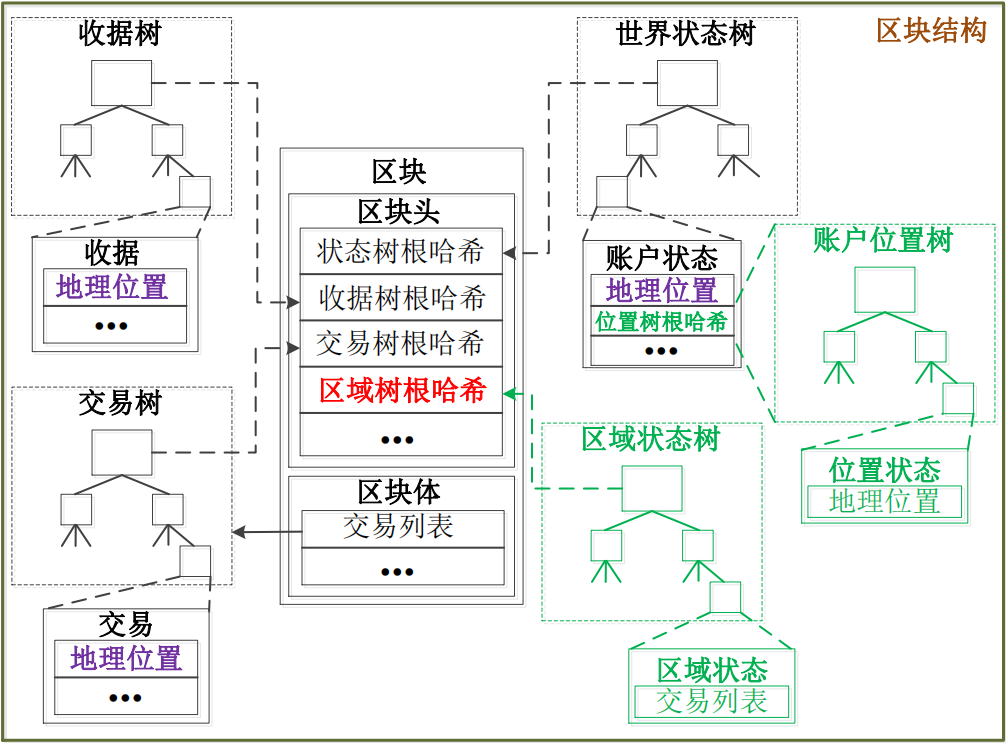
\includegraphics[width=0.7\textwidth]{images/区域链区块示意图.png}
  \caption{区域链区块示意图}\label{区域链区块示意图} % label 用来在文中索引
\end{figure}

区域索引区块链仍然保留了传统区块链的单链结构,当区块数量很大时,其查询效率仍然会随之降低。因此,周畅提出并设计了基于区域索引区块链改良的树状区域索引区块链(下简称树状区块链)。其按照Geohash编码长度,表示父链和子链的关系,并划分区域子链。树状区块链的区块也分为三种:叶子区块、分支区块和创世块。叶子区块和传统的区块链并无太大差异,叶子区块及其后续区块均采用传统的单链结构加以组织;分支区块则负责将数个叶子区块组织起来,按照叶子区块所代表的地理位置,创世块和分支区块十分相似,但它没有父链指针。上述树状区块链的设计,进一步缩短了区块链网络中的单链长度,进而提升了查询效率。

\subsection{以太坊和Substrate}
% 顺手介绍一下以太坊和Substrate

中本聪提出的比特币区块链系统支持简单的基于栈的编程语言,由于其并非图灵完备(例如不支持循环等结构),程序员仅能在其上进行受限的操作,这很大程度上限制了区块链技术的应用场景。以太坊\cite{ethereumWhitePaper}技术的诞生,旨在提出一种建立分布式应用程序(又名去中心化应用程序,DApps)的新方法,其提供名为以太坊虚拟机(EVM),采用图灵完备的编程语言,令程序员得以编写更复杂更强大的智能合约,进而根据实际需求灵活定制状态转换函数等功属性。

以太坊技术的成熟引领人们走进了Web 2.0时代。然而,随着以太坊在各行各业使用愈加广泛,其局限性亦逐渐显露。简而言之,以太坊为保证其功能全面性,其官方实现非常复杂且可扩展性不足,导致程序体积巨大、运行效率低下、且核心定制变得尤为繁琐。Substrate提出了一种模块化的区块链构建框架,允许程序员自行选用充分必要的模块构建更贴近实际需求,拥有更少多余功能的区块链。此外,Substrate选用Rust编程语言作为其底层实现,令区块链在WebAssembly上运行成为可能。由于现代浏览器普遍支持WebAssembly,这意味着区块链的运行环境终于从以太坊虚拟机(EVM)中解放出来,可以在浏览器中直接运行,不仅程序运行速度更快,且跨平台兼容性大大提升。

\section{本文研究内容及贡献}

本文将在车联网这一应用场景下,首先基于区域索引区块链,复现实验室已有工作——出租车调度系统的有关工作,证明该系统的可用性。此后,设计并进行树状区域索引区块链在单父链双子链的网络结构下的跨链转账实验,探究树状区块链在不同转账请求压力下的性能表现,验证其功能可用性,并测试跨链操作带来的额外时间开销。作为测试实验的收尾,本文将设计实验,令出租车调度系统分别在网络结构不同的树状区块链上运行,收集并可视化实验数据,评估树状区块链在不同工况的实际应用场景下的性能表现。本文还将为树状区块链从以太坊平台转向更优秀的Substrate平台做出积极探索。鉴于时间和笔者能力之限,本文仅讨论区域索引区块链的部分功能特性的迁移工作,此举旨在验证两平台在功能上相似,进而证明未来树状区块链的底层功能迁移工作的可行性。

\begin{enumerate}
  \item 基于区域索引区块链,复现实验室已有工作——出租车调度系统,证明该系统的可用性;编写帮助文档和实验日志,以便后人推进研究
  \item 设计并进行树状区域索引区块链在单父链双子链的网络结构下的跨链转账实验,记录其对10个、20个、40个、80个、120个、160个、200个账号执行子链之间的跨链转账的耗时、吞吐量等数据,并进行可视化;编写帮助文档和实验日志,以便后人推进研究
  \item 在单子链、单父链四子链的网络结构下分别运行出租车调度系统,探究树状区块链在不同工况实际场景中的性能表现,并进行数据可视化;编写帮助文档和实验日志,以便后人推进研究
  \item 探索区域索引区块链的部分功能特性从以太坊向Substrate的迁移的可行性,为Substrate的官方实现引入账户地理位置这一字段,令其可以在创世块配置文件中修改、在账户查询时显示;编写实验日志,以便纠错和改进
\end{enumerate}


% \textcolor{blue}{公式标注应于该公式所在行的最右侧。对于较长的公式只可在符号处(+、-、*、/、$\leqslant$ $\geqslant$ 等)转行。在文中引用公式时,在标号前加“式”,如式(1-2)。阅后删除此
%   段。}

% \textcolor{blue}{公式-示例:(阅后删除此段)}
% % 公式上下不要空行,置于同一个段落下即可,否则上下距离会出现高度不一致的问题
% \begin{equation}
%   LRI=1\ ∕\ \sqrt{1+{\left(\frac{{\mu }_{R}}{{\mu }_{s}}\right)}^{2}{\left(\frac{{\delta }_{R}}{{\delta }_{s}}\right)}^{2}}
% \end{equation}

% \subsubsection{生僻字}

% 一个可能无法正常显示的生僻字
% 一个可能无法正常显示的生僻字: 彧。下文注释中,介绍了如何通过自定义字体来显示生僻字。

% 定义一个提供了生僻字的字体,注意要确保你的系统存在该字体
% \setCJKfamilyfont{custom-font}{Noto Serif CJK SC}

% 使用自己定义的字体
% 使用提供了相应字型的字体:\CJKfamily{custom-font}{彧}。

